\documentclass{beamer}
%
% Choose how your presentation looks.
%
% For more themes, color themes and font themes, see:
% http://deic.uab.es/~iblanes/beamer_gallery/index_by_theme.html
%
\mode<presentation>
{
  \usetheme{Berkeley}      % or try Darmstadt, Madrid, Warsaw, ...
  \usecolortheme{dove} % or try albatross, beaver, crane, ...
  \usefonttheme{default}  % or try serif, structurebold, ...
  \setbeamertemplate{navigation symbols}{}
  \setbeamertemplate{caption}[numbered]
} 

\usepackage[finnish]{babel}
\usepackage[utf8x]{inputenc}
\usepackage{pgfgantt}
\usepackage{graphicx}
\usepackage{csquotes}

\title[JOTU-2019 Megantti]{Megantti konsernin asiakastietojärjestelmä}
\author{Ryhmä 39}
\institute{Tampereen Teknillinen Yliopisto}
\date{\today}

\begin{document}

\begin{frame}
  \titlepage
\end{frame}

% Uncomment these lines for an automatically generated outline.
\begin{frame}{Tänään käsittelemme}
	\tableofcontents[pausesections]
\end{frame}

\section{Johdanto}

\begin{frame}{Esittely}
\begin{itemize}
  \item<1-> Me olemme
  \item<2-> Megantti on kansallinen kodinkoneita ja elektroniikkaa myyvä konserni
\end{itemize}

\begin{figure}

\includegraphics[scale=0.65]{../megantti.png}
	\caption{Megantti konsernin logo}
\end{figure}

\end{frame}

\begin{frame}{Harjoitustyön kulku}
	\begin{itemize}
		\item<2-> Gitissä 120+ committia
		\item<3-> Aktiivinen ryhmätyöskentely
		\item<4-> noin 12 kahvipannullista per viikko
		\item<5-> 150+ miestyötuntia (vscoden työaikalaskurin mukaan)
	\end{itemize}
\end{frame}


\section{Megantti konsernin CRM}


\subsection{CRM esittely}

\begin{frame}{Millainen on hyvä CRM?}

Hyvän CRM piirteitä

	\begin{itemize}
		\item<2-> Helppokäyttöinen
		\item<3-> Nopea
		\item<4-> Yhteensopiva
		\item<5-> Luotettava
	\end{itemize}
\end{frame}

\subsection{Esimerkki\-käyttäjä\-tapaus}

\begin{frame}{Käyttötapauskaaviot}

	\begin{figure}[h]
		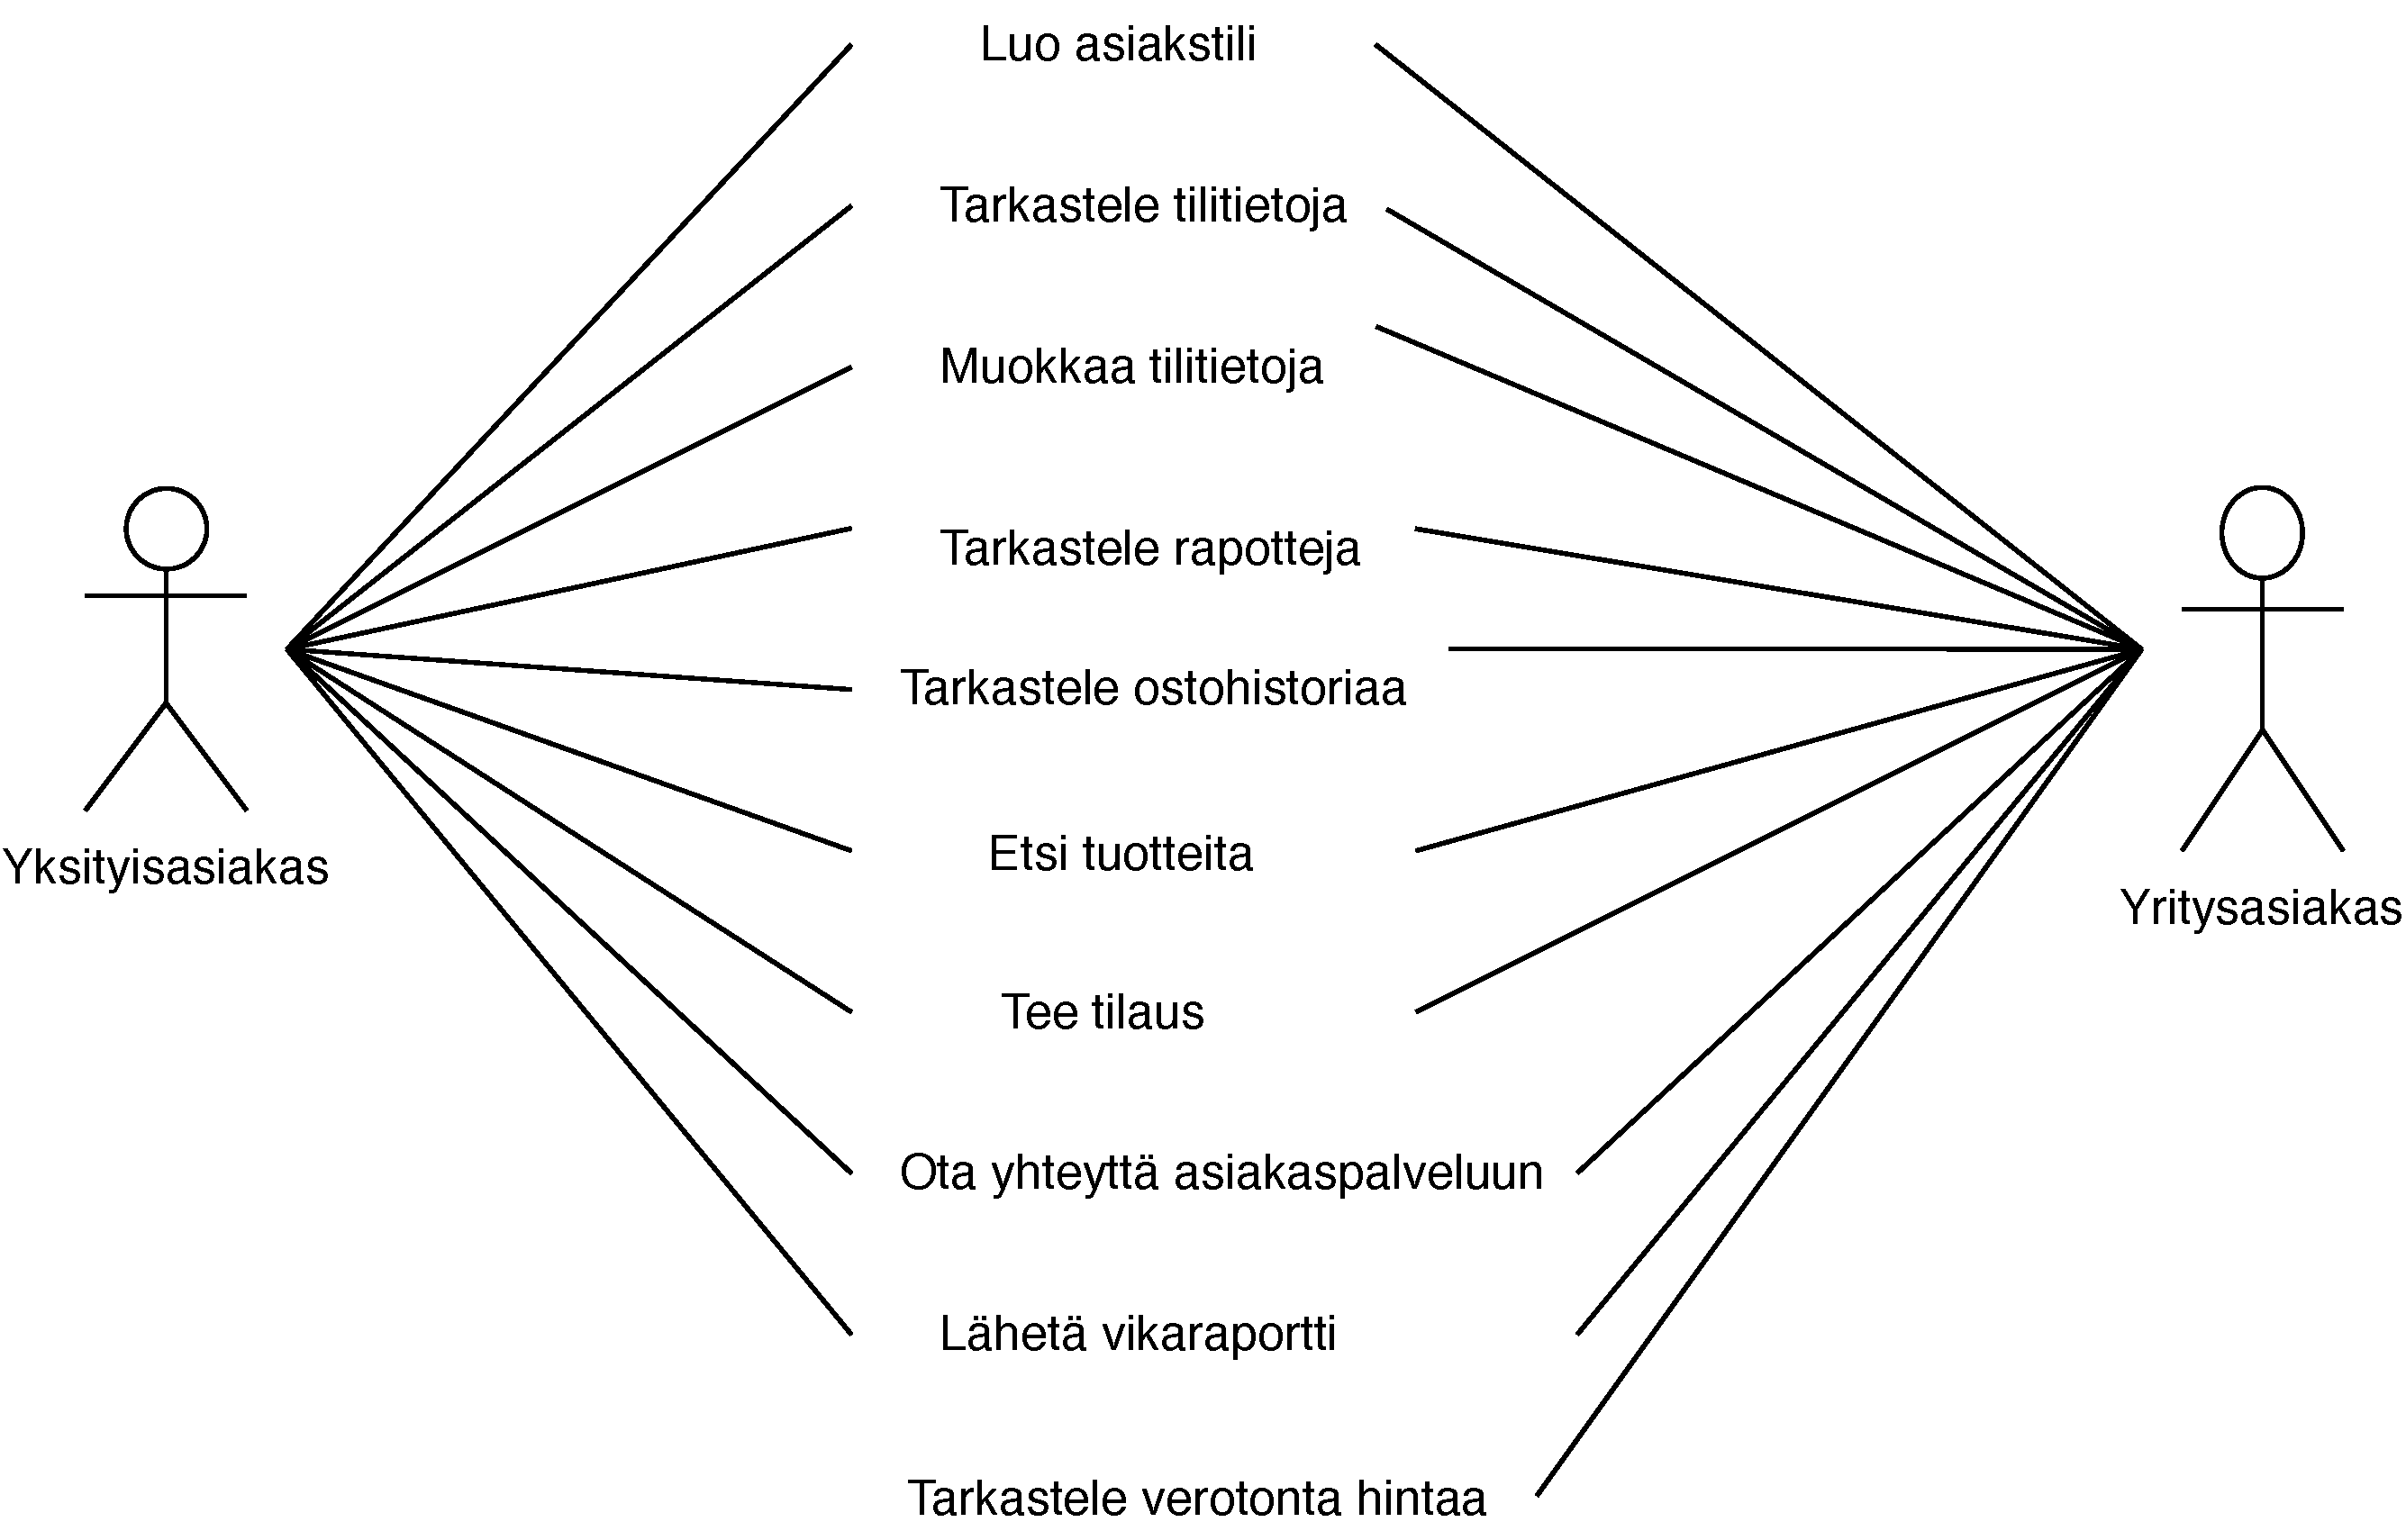
\includegraphics[width=0.8\textwidth]{../harjoitustyo/images/kayttotapauskaavio1.pdf}
		\caption{Käyttötapauskaavio 1 - Asiakas}
	\end{figure}

\end{frame}

\begin{frame}{Käyttötapauskaaviot}

	\begin{figure}[h]
		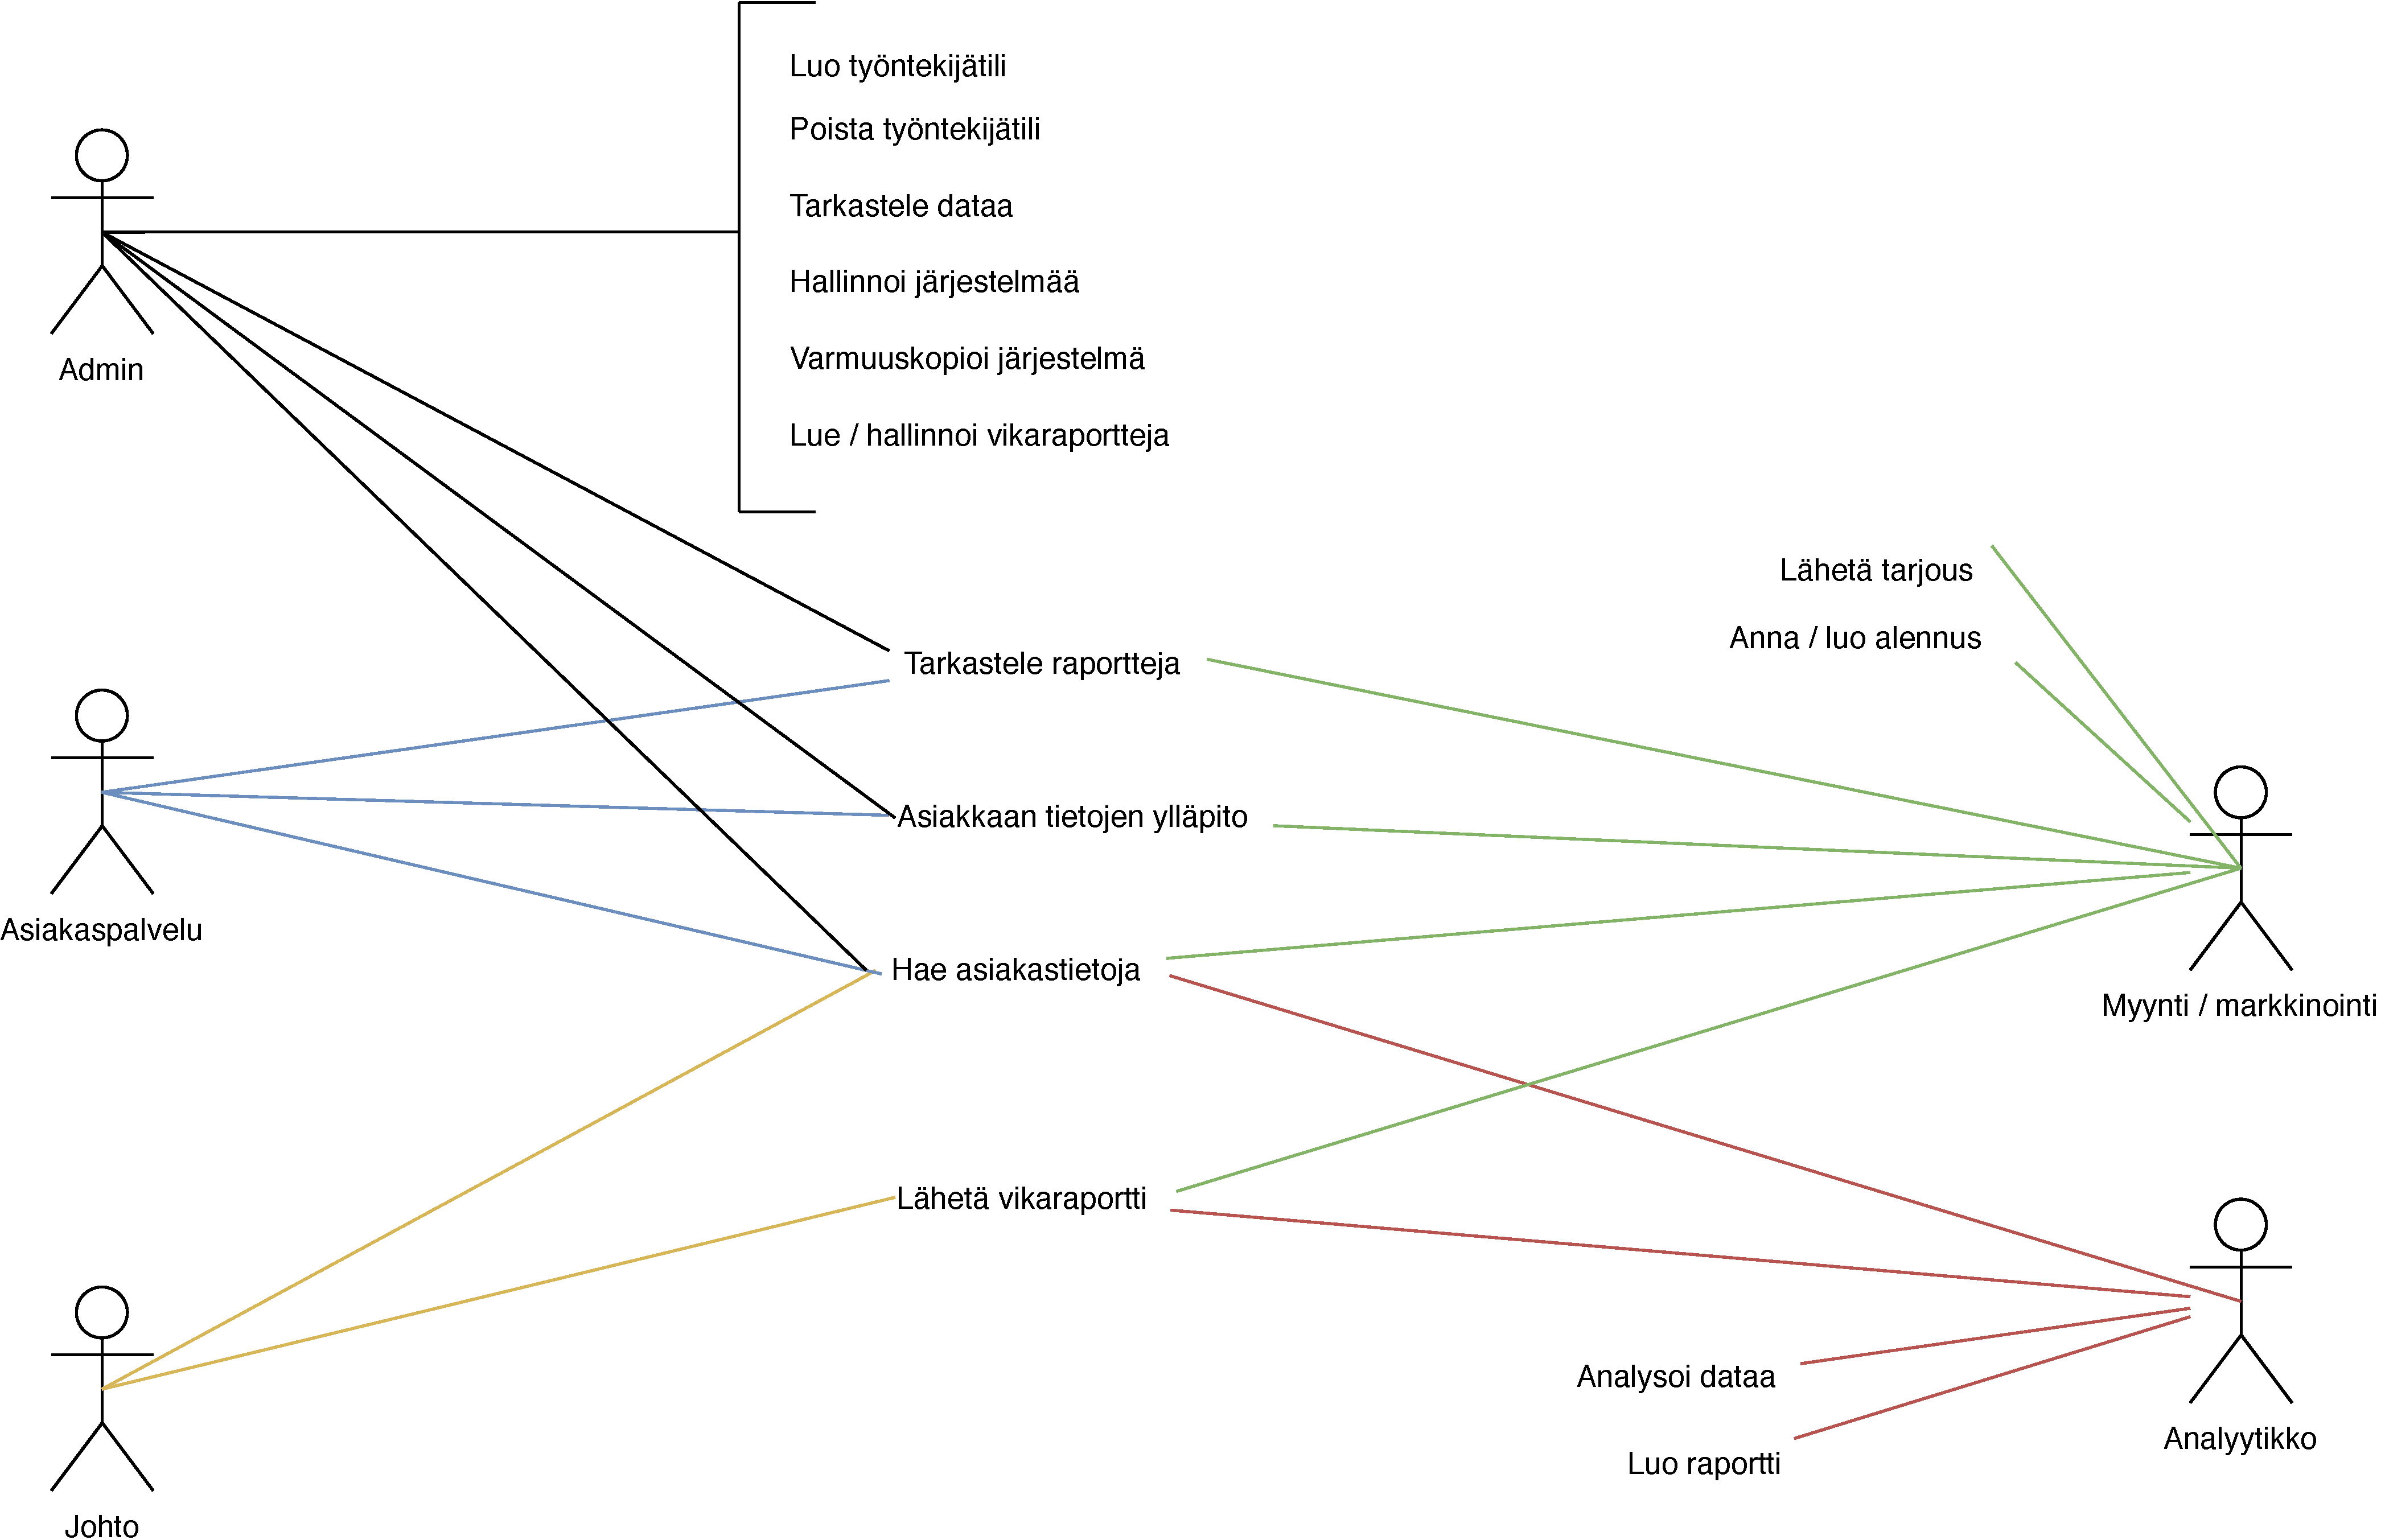
\includegraphics[width=0.8\textwidth]{../harjoitustyo/images/kayttotapauskaavio2.pdf}
		\caption{Käyttötapauskaavio 2 - Sisäiset toimijat}
	\end{figure}

\end{frame}

\begin{frame}{Esimerkkikäyttäjätapaus}
	\begin{enumerate}
		\item Järjestelmä ehdottaa tiettyä asiakasryhmää koskevaa alennusta.
		\item Alennuksesta määritellään sen suuruus ja kesto sekä tuoteryhmät, joita alennus koskee.
		\item Alennus perustuu järjestelmän sisäisiin statistiikkoihin.
		\item Mikko Myyntitykki voi valita, hyväksyykö hän ehdotetun tarjouksen vai ei.
		\item Hän voi myös määritellä alennuksen itse niin halutessaan.
			\begin{itemize}
				\item Erittäin suuria alennuksia luotaessa tulostetaan varoitus.
			\end{itemize}
		\item Valmiista alennuksesta lähetetään asiakkaalle sähköinen ilmoitus.
	\end{enumerate}
	
\end{frame}


\subsection{Järjestelmän rakenne}

\begin{frame}{Lopulliset vaatimukset}

\begin{table}[]
\resizebox{\textwidth}{!}{% use resizebox with textwidth
    \begin{tabular}{lllll}
		\multicolumn{4}{l}{Prioriteeti (1=Vähiten tärkeä, 2= Jonkin verran tärkeä, 3= Erittäin tärkeä)  Luokat (T=Tuottajat, H=Hyödyntäjät, J=Järjestelmävaatimus)}                                                                                                                                                                           \\ \hline
		\multicolumn{1}{|l|}{1}		&			 \multicolumn{1}{|l|}{{\color[HTML]{000000} \textbf{Prioriteetti}}} & \multicolumn{1}{l|}{{\color[HTML]{000000} \textbf{Lähde}}} & \multicolumn{1}{l|}{{\color[HTML]{000000} \textbf{Luokka}}} & \multicolumn{1}{l|}{{\color[HTML]{000000} \textbf{Vaatimus}}}                                                \\ \hline
    \multicolumn{1}{|l|}{2}		&			 \multicolumn{1}{|l|}{3}& \multicolumn{1}{l|}{Taustatutkimus}			& \multicolumn{1}{l|}{T/H}                                    & \multicolumn{1}{l|}{Järjestelmän tulee noudattaa GDPR:ää.}                                                   \\ \hline
    \multicolumn{1}{|l|}{3}		&			 \multicolumn{1}{|l|}{3}& \multicolumn{1}{l|}{Haastattelut}				& \multicolumn{1}{l|}{J}                                    & \multicolumn{1}{l|}{Asiakastietojärjestelmää tulee pystyä käyttää eri päätelaitteilta.}                       \\ \hline
    \multicolumn{1}{|l|}{4}		&			 \multicolumn{1}{|l|}{3}& \multicolumn{1}{l|}{Taustatutkimus}			& \multicolumn{1}{l|}{J}                                      & \multicolumn{1}{l|}{Järjestelmän tulee olla yhteensopiva muiden olemassa olevien järjestelmien kanssa.}      \\ \hline
    \multicolumn{1}{|l|}{5}		&			 \multicolumn{1}{|l|}{2}& \multicolumn{1}{l|}{Havainnointi}				& \multicolumn{1}{l|}{T}                                      & \multicolumn{1}{l|}{Asiakkaiden tiedot tulee pystyä etsiä järjestelmästä nopeasti.}                           \\ \hline
    \multicolumn{1}{|l|}{6}		&			 \multicolumn{1}{|l|}{3}& \multicolumn{1}{l|}{Haastattelut}				& \multicolumn{1}{l|}{J}                                      & \multicolumn{1}{l|}{Järjestelmä rakennetaan olemassa olevan olevan ERP SQL constructoreiden päälle.}          \\ \hline
    \multicolumn{1}{|l|}{7}		&			 \multicolumn{1}{|l|}{2}& \multicolumn{1}{l|}{Prototyypit}				& \multicolumn{1}{l|}{T}                                      & \multicolumn{1}{l|}{Järjestelmän tulee seurata asiakkaiden ostoskäyttäytymistä.}                              \\ \hline
    \multicolumn{1}{|l|}{8}		&			 \multicolumn{1}{|l|}{3}& \multicolumn{1}{l|}{Havainnointi}				& \multicolumn{1}{l|}{T}                                      & \multicolumn{1}{l|}{Järjestelmän tulee pitää lokia kaikista tapahtumista.}                                   \\ \hline
    \multicolumn{1}{|l|}{9}		&			 \multicolumn{1}{|l|}{2}& \multicolumn{1}{l|}{Taustatutkimus}			& \multicolumn{1}{l|}{T}                                      & \multicolumn{1}{l|}{Järjestelmän pitää pystyä analysoida ja profiloida asiakkaita.}                         \\ \hline
    \multicolumn{1}{|l|}{10}		&			 \multicolumn{1}{|l|}{1}& \multicolumn{1}{l|}{Prototyypit/Haastattelut}& \multicolumn{1}{l|}{T/H}                                    & \multicolumn{1}{l|}{Järjestelmän tulee olla helppokäyttöinen(Graphical user Interface.)}                    \\ \hline
    \multicolumn{1}{|l|}{11}		&			 \multicolumn{1}{|l|}{1}& \multicolumn{1}{l|}{Prototyypit}			& \multicolumn{1}{l|}{J}                                    & \multicolumn{1}{l|}{Järjestelmässä tulee olla monipuolisia toimintoja, kuten ostoshistoria, selainhistoria.}\\ \hline
    \multicolumn{1}{|l|}{12}		&			 \multicolumn{1}{|l|}{2}& \multicolumn{1}{l|}{Haastattelut}			& \multicolumn{1}{l|}{J}                                    & \multicolumn{1}{l|}{Järjestelmän luotettavuus tulee taata.}                                                 \\ \hline
    \multicolumn{1}{|l|}{13}		&			 \multicolumn{1}{|l|}{1}& \multicolumn{1}{l|}{Ryhmätapaamiset}	& \multicolumn{1}{l|}{H}                                    & \multicolumn{1}{l|}{Järjestelmän tulee pystyä yksilöllistää asiakkaan markkinointia.}                       \\ \hline
		\multicolumn{1}{|l|}{14}		&			 \multicolumn{1}{|l|}{2}& \multicolumn{1}{l|}{Ryhmätapaamiset}	& \multicolumn{1}{l|}{T}                                    & \multicolumn{1}{l|}{Järjestelmän tulee pitää kirjaa järjestelmätapahtumista.}                               \\ \hline
		\multicolumn{1}{|l|}{15}		&			 \multicolumn{1}{|l|}{2}& \multicolumn{1}{l|}{Taustatutkimus}	& \multicolumn{1}{l|}{J}                                    & \multicolumn{1}{l|}{Järjestelmän backendin tulee olla erotettu frontendistä (headless)}                               \\ \hline
		\multicolumn{1}{|l|}{16}		&			 \multicolumn{1}{|l|}{3}& \multicolumn{1}{l|}{Haastattelut}	& \multicolumn{1}{l|}{J}                                    & \multicolumn{1}{l|}{Järjestelmällä tulee olla web pohjainen skaalautuva käyttöliittymä}                               \\ \hline
		\multicolumn{1}{|l|}{17}		&			 \multicolumn{1}{|l|}{3}& \multicolumn{1}{l|}{Ryhmätapaamiset}	& \multicolumn{1}{l|}{H}                                    & \multicolumn{1}{l|}{Asiakkaan tulee osata käyttää järjestelmää ilman alustavaa koulutusta}                               \\ \hline
		\multicolumn{1}{|l|}{18}		&			 \multicolumn{1}{|l|}{3}& \multicolumn{1}{l|}{Prototyypit}	& \multicolumn{1}{l|}{J}                                    & \multicolumn{1}{l|}{Headless frontin API:n tulee käyttää HSTS menetelmää}																	\\ \hline
		\multicolumn{1}{|l|}{19}		&			 \multicolumn{1}{|l|}{3}& \multicolumn{1}{l|}{Taustatutkimus}	& \multicolumn{1}{l|}{H}                                    & \multicolumn{1}{l|}{Asiakastietojärjestelmän on automatisoitava varmuuskopiointi}								\\ \hline
		\multicolumn{1}{|l|}{20}		&			 \multicolumn{1}{|l|}{2}& \multicolumn{1}{l|}{Ryhmätapaamiset}	& \multicolumn{1}{l|}{J}                                    & \multicolumn{1}{l|}{Asiakastietojärjestelmästä on oltava dokumnentaatio}														\\ \hline
		\multicolumn{1}{|l|}{21}		&			 \multicolumn{1}{|l|}{2}& \multicolumn{1}{l|}{Taustatutkimus}	& \multicolumn{1}{l|}{J}                                    & \multicolumn{1}{l|}{Järjestelmän tietoja tulee pystyä editoimaan CRUD-menetelmän mukaisesti, jokaisen clientin kautta}									\\ \hline
		\multicolumn{1}{|l|}{22}		&			 \multicolumn{1}{|l|}{3}& \multicolumn{1}{l|}{Taustatutkimus}	& \multicolumn{1}{l|}{J}                                    & \multicolumn{1}{l|}{Järjestelmässä tulee olla selkeä \textit{Access policy} käyttäjille}						\\ \hline
		\multicolumn{1}{|l|}{23}		&			 \multicolumn{1}{|l|}{2}& \multicolumn{1}{l|}{Taustatutkimus}	& \multicolumn{1}{l|}{H}                                    & \multicolumn{1}{l|}{Asiakas tulee pystyä etsiä järjestelmästä mahdollisimman monen tietoyhteyden avulla}						\\ \hline
		                     
		
   

    \end{tabular}
}
    \caption{Taulukko keskeisistä vaatimuksista}
    \label{tab:vaatimukset}
    \end{table}
\end{frame}

\subsection{Tietoyhteydet järjestelmän sisällä}

\begin{frame}{Tietoyhteydet järjestelmän sisällä}


	\begin{figure}[h]
		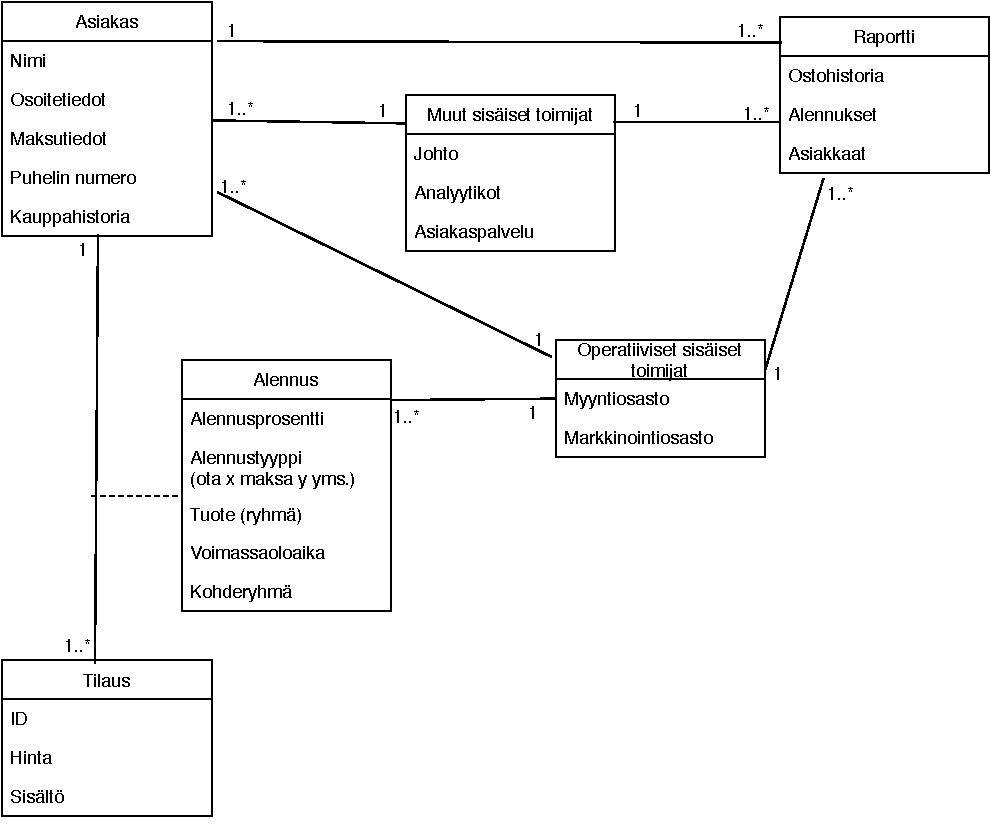
\includegraphics[width=0.8\textwidth]{../harjoitustyo/images/Tietoyhteyskaavio.pdf}
		\caption{Tietoyhteyskaavio}
	\end{figure}

\end{frame}


\subsection{Esimerkki käyttöliittymästä}

\begin{frame}{Tältä käyttöliittymä voisi näyttää}

	\begin{figure}[h]
		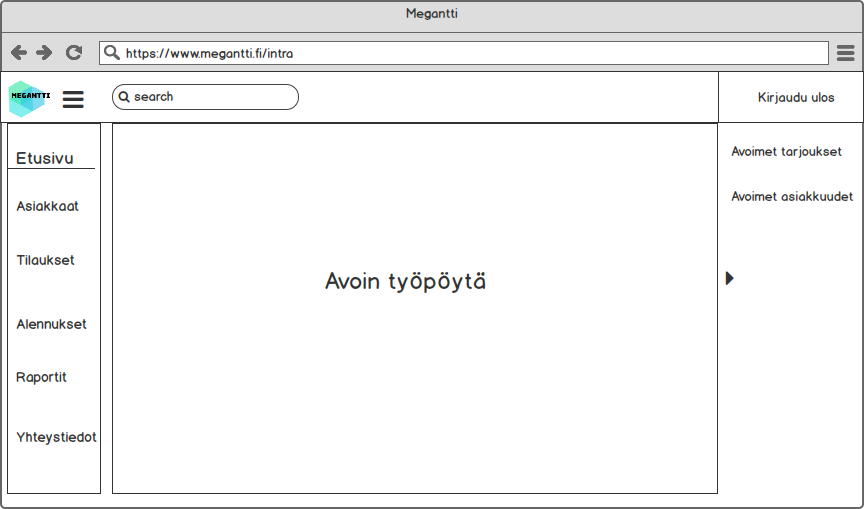
\includegraphics[width=\textwidth]{../harjoitustyo/images/gui/sisainen_paa.png}
		\caption{Sisäisen käyttäjän päänäkymä}
	\end{figure}

\end{frame}

\section{Lopuksi}

\begin{frame}{Loppusanat}

	\begin{displayquote}
		"Hyvin suunniteltu on puoliksi tehty, ja puoliksi tehty on kelvannut ennenkin."
	\end{displayquote}

\end{frame}


\begin{frame}

\end{frame}

\end{document}
